\documentclass{standalone}
\usepackage{tikz}
\tikzset{ block/.style = {draw, fill=white, very thick, rectangle, minimum height=1cm, minimum width=2cm},}
\tikzset{sum/.style= {draw, fill=white, very thick, circle, node distance=1cm},}
\begin{document}
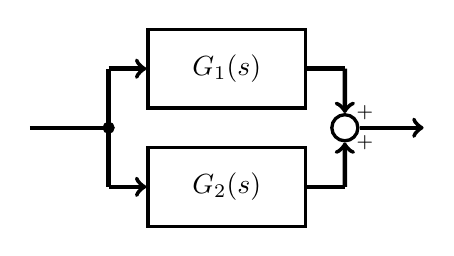
\begin{tikzpicture}[scale=2]
    \node[block, node distance=0cm](g1){$G_1(s)$};
    \node[block, below of=g1, node distance=1.5cm](g2){$G_2(s)$};
    \filldraw[black](-0.75,-0.375)circle(1pt)coordinate(split);
    \node[sum, right of=split, node distance=3cm](sum){};
    \draw[-,ultra thick](-1.25,-0.375)--(-0.75,-0.375);
    \draw[-,ultra thick](split)--(-0.75,0);
    \draw[-,ultra thick](split)--(-0.75,-0.75);
    \draw[->,ultra thick](-0.75,0)--(g1.180);
    \draw[->,ultra thick](-0.75,-0.75)--(g2.180);
    \draw[-,ultra thick](g1.0)--(0.75,0);
    \draw[-,ultra thick](g2.0)--(0.75,-0.75);
    \draw[->,ultra thick](0.75,0)--(sum.90)node[right]{$_{+}$};
    \draw[->,ultra thick](0.75,-0.75)--(sum.270)node[right]{$_{+}$};
    \draw[->,ultra thick](sum.0)--(1.25,-0.375);
\end{tikzpicture}
\end{document}